Luminosity in the database dataset will be measured with gamgams
because $e^+e^-$ and $\mu^+\mu^-$ are both final states of the
$\Upsilon$.  But can any $\Upsilon$ decays pass gamgam cuts?  Gamgam
requires two large, back-to-back showers, and $\Upsilon \to
\gamma\gamma$ is forbidden by angular momentum conservation.  But
$\chi_{b0}$ and $\chi_{b2}$ are $J^{PC}$ = $0^{++}$ and $2^{++}$
particles, respectively, and can therefore decay to $\gamma\gamma$.
One can imagine, then, a cascade in which the $\Upsilon$ radiates a
small photon to become a $\chi_b$, and then the $\chi_b$ decays into
two large, back-to-back photons.  Such an event would pass gamgam cuts
because gamgam does not exclude a small third photon.

To check for this possibility, I searched the database dataset for
events of this type.  In $\Upsilon(2S)$ and $\Upsilon(3S)$
on-resonance and off-resonance data, I plotted the third largest
shower energy (\ethree) for all events that satisfy gamgam cuts in
Figure \ref{gamgam_chibkgnd}.  The lowest energy a $\Upsilon \to
\chi_b$ cascade photon can have is 60 MeV, so I used gamgam events
with \ethree\ $<$ 60 MeV to scale the off-resonance sample.  Rather
than subtracting on- and off-resonance, I have overlaid them.  Monte
Carlo for this decay chain has also been overlaid (with an arbitrary
normalization) to show where \ethree\ peaks can be expected.  (The
Monte Carlo includes $\chi_{b1}$ in the cascade chain.)  No peaks are
seen in data in the right places.  The differences between on- and
off-resonance distributions are due to variations in noise that do not
affect gamgam counting.

\begin{figure}
  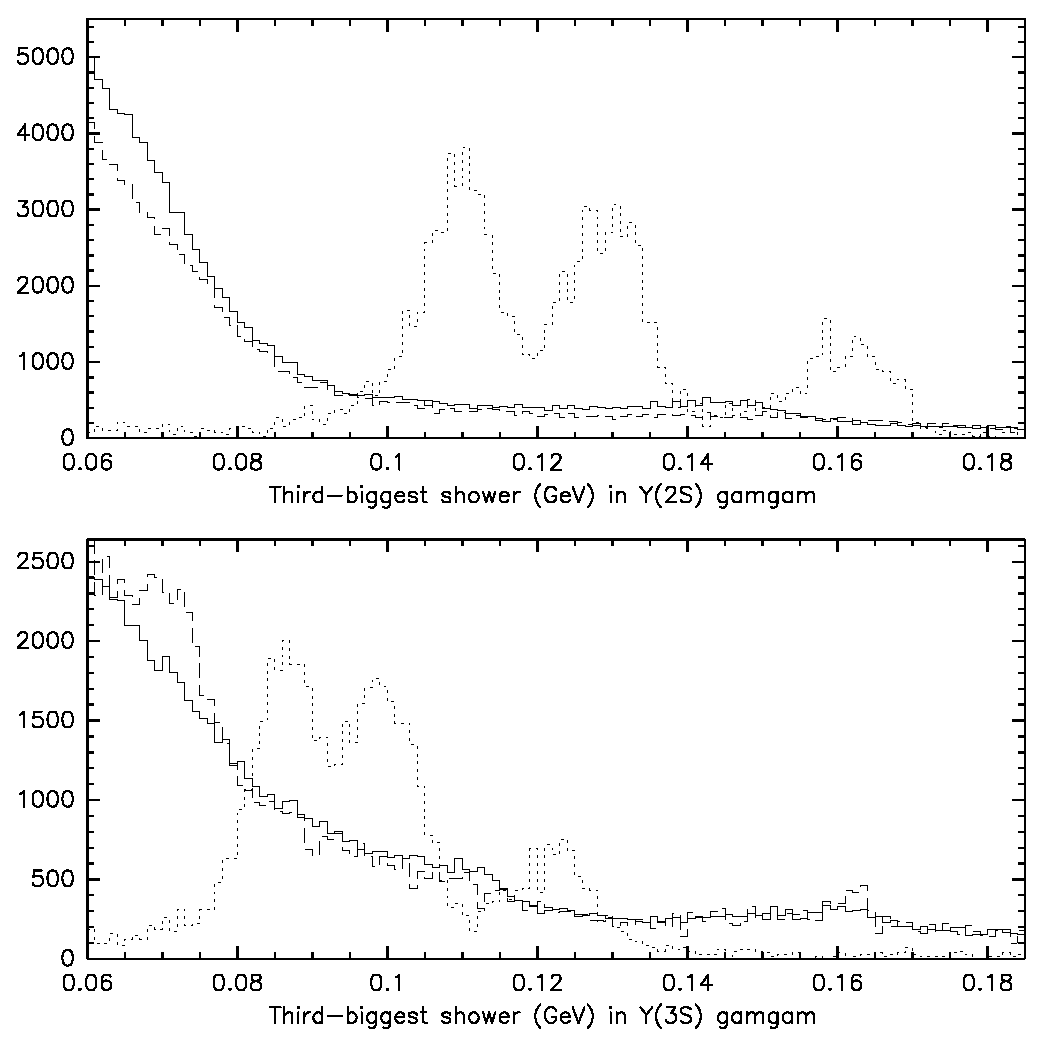
\includegraphics[width=\linewidth]{plots/gamgam_chibkgnd}
  \caption{\label{gamgam_chibkgnd} Energy of the third-largest shower
    in gamgam events.  On-resonance data are solid, scaled
    off-resonance data are dashed, and $\Upsilon \to \gamma
    \chi_{b0,1,2} \to \gamma \gamma \gamma$ Monte Carlo are dotted.}
\end{figure}

Since the database dataset is insensitive to this decay mode, any bias
due to $\gamma\gamma\gamma$ events must be smaller than statistical
errors in the luminosity measurement.  I will ignore its contribution.
